% This example is meant to be compiled with lualatex or xelatex
% The theme itself also supports pdflatex
\PassOptionsToPackage{unicode}{hyperref}
\documentclass[aspectratio=1610, 9pt]{beamer}

% Load packages you need here
\usepackage{polyglossia}
\setmainlanguage{german}

\usepackage{csquotes}
    

\usepackage{amsmath}
\usepackage{amssymb}
\usepackage{mathtools}

\usepackage{hyperref}
\usepackage{bookmark}

% load the theme after all packages

\usetheme[
  showtotalframes, % show total number of frames in the footline
]{tudo}

% Put settings here, like
\unimathsetup{
  math-style=ISO,
  bold-style=ISO,
  nabla=upright,
  partial=upright,
  mathrm=sym,
}

%Titel:
\title{Radiolaute aktive Galaxienkerne}
%Autor
\author[N.Breer]{Nils Breer}
%Lehrstuhl/Fakultät
\institute{Fakultät Physik}
%Titelgrafik muss ich einfueren!!!
%\titlegraphic{\includegraphics[width=0.3\textwidth]{content/Bilder/interferenz.jpg}}
\date{28.11.2019}

\begin{document}
\maketitle

\begin{frame}\frametitle{Agenda}
  \begin{itemize}
    \item Historie und Entdeckung der AGN
    \item Aufbau und Klassifizierung von AGN
    \item 
    \item Detektion von AGN
    \item Fazit
  \end{itemize}
\end{frame}

\begin{frame}\frametitle{Historie und Entdeckung}
  \begin{itemize}
    \item 1908, Fath: Anormales Spektrum von Spiralnebeln
    \item 1943, Seyfert: helle, sternartige Kerne mit breiten Emissionslinien
    \item 1954: Cygnus A als erste Radiogalaxie identifiziert
    \item nach 1960: nuche nach weiteren Radiogalaxien mit bestimmten Kriterien.
    \item 3C 273: Emissionslinie stark verschoben $\to$ gro\ss e Rotverschiebung
  \end{itemize}
\end{frame}

% bild einfuegen

\begin{frame}\frametitle{Aufbau und Klassifizierung von AGN}
  \begin{block}{Aufbau und Annahmen}
  \begin{columns}
  \begin{column}[c]{0.45\textwidth}
  \begin{itemize}
    \item Staubtorus
    \item SMBH
    \item Akkretions-Scheibe
    \item Jets
    \item breites Emissionsspektrum an nicht-thermischer Strahlung
    \item schnelle Variabilit\"at
    \item kleines Emissionsgebiet (Jetorigin) ~ 7 AE
    \item schnelle Rotation von Gas um Zentrum ~ einige AE
    \item hohe Geschwindigkeiten $\to$ hohe Masse (M87 SMBH)
  \end{itemize}
  \end{column}
  \begin{column}[c]{0.45\textwidth}
    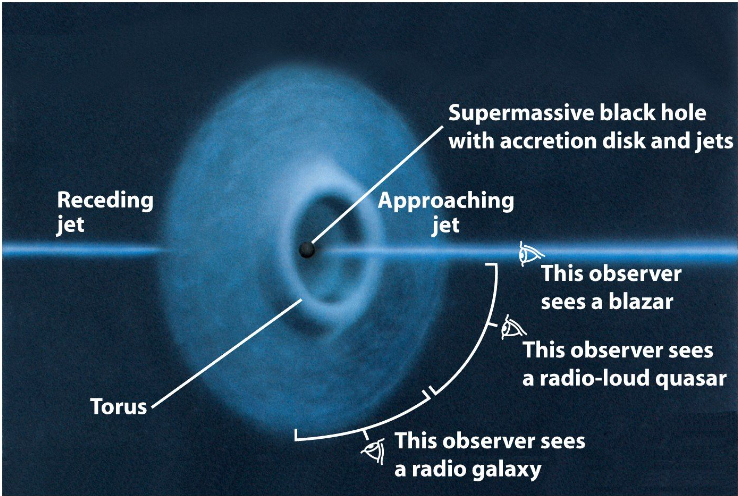
\includegraphics{images/agn-pic.png}
  \end{column}
  \end{columns}
  \end{block}
\end{frame}

\begin{frame}\frametitle{Aufbau und Klassifizierung von AGN}
  \begin{block}{Typen von AGN}
    \begin{itemize}
      \item Seyfert-Galaxien
      \item Radiogalaxien
      \item Quasare (quasi stellar radio sources)
      \item Blazare
      \item Fanaroff-Riley Galaxien
    \end{itemize}
  \end{block}
\end{frame}


\begin{frame}\frametitle{Seyfert-Galaxien}
  \begin{itemize}
    \item ca. 90 \% sind Spiralgalaxien
    \item h\"aufigster Galaxientyp mit AGN
    \item Heller, blauer Kern
    \item Emissionslinie f\"uhrt auf hei\"sses ionisiertes Gas
    \item Helligkeits\"anderung des Kerns schnell (f\"ur astronomische Zeitskalen)
    \item Hoher Geschindigkeit des Gases im Zentrum der Galaxie
    \item aber nur radioleiser Galaxientyp
  \end{itemize}
\end{frame}

\begin{frame}\frametitle{Fanaroff-Riley Galaxien}
  \begin{block}{FR Typ 1}
  \begin{columns}
  \begin{column}{0.45\textwidth}
    \begin{itemize}
      \item Radioemission ~ 1/r
      \item h\"aufig Back to Back Jets
    \end{itemize}
  \end{column}
  \begin{column}{0.45\textwidth}
    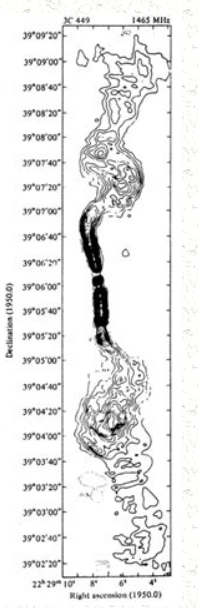
\includegraphics{images/FR1.png}
      % hier ein bild von FR1 1 einfuegen
  \end{column}
  \end{columns}
  \end{block}
\end{frame}

\begin{frame}\frametitle{Fanaroff-Riley Galaxien}
  \begin{block}{FR Typ 2}
  \begin{columns}
  \begin{column}[c]{0.45\linewidth}
    \begin{itemize}
      \item Helle "Hot Spots" in Keulen
      \item relativ dunkler Kern
      \item oft einseitiger Jet
      \item i.A. heller als FR-1 durch Keulen
    \end{itemize}
  \end{column}
  \begin{column}[c]{0.45\linewidth}
    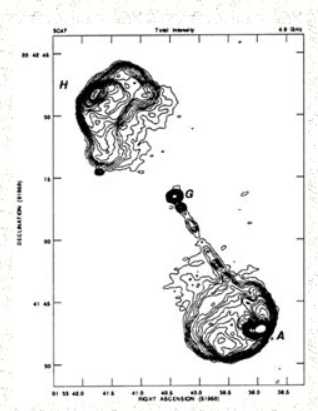
\includegraphics{images/FR2.png}
      % hier ein bild von FR1 1 einfuegen
  \end{column}
  \end{columns}
  \end{block}
\end{frame}

\begin{frame}\frametitle{Blazare}
  \begin{block}{Typen}
  \begin{columns}
  \begin{column}[c]{0.45\linewidth}
    \begin{itemize}
      \item Flat Spektrum Radio Quasars
      \item Doppelh\"ocker Struktur
      \item BL Lacertae-artig
      \begin{itemize}
        \item ver\"anderlicher Stern (Cuo Hoffmeister, Sternbild Eidechse)
        \item Blick direkt in Jetachse
      \end{itemize}
    \end{itemize}
    \end{column}
    \begin{column}[c]{0.45\linewidth}
      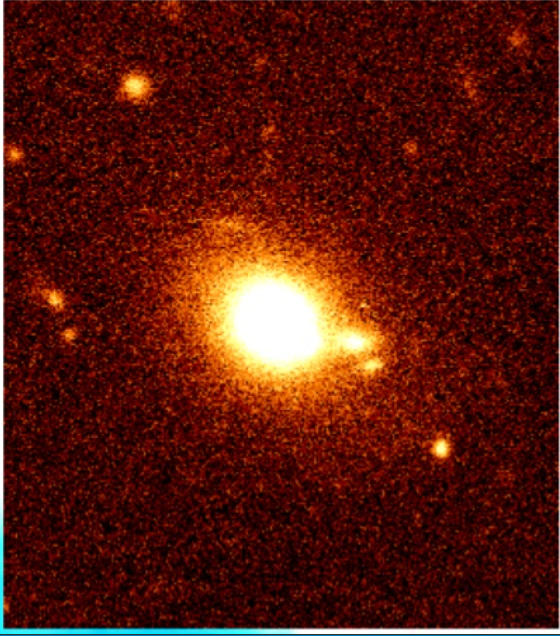
\includegraphics{images/bl-lac-object.png}
    \end{column}
    \end{columns}
  \end{block}
\end{frame}

\begin{frame}\frametitle{Jet Modelle}
  \begin{columns}
  \begin{column}[c]{0.45\linewidth}
  \begin{itemize}
    \item Synchrotron-Self-Compton Modell
    \begin{itemize}
      \item Synchrotron Emission durch $e^{-}$, first Bump
      \item HE Bump: inverser Compton Effekt mit eigenen Photonen
      \item h\"aufig f\"ur BL Lacertae Spektren
    \end{itemize}
    \item External Compton Modell
    \begin{itemize}
      \item Synchrotron Emission durch $e^{-}$, first Bump
      \item HE Bump: inverser Compton Effekt mit eigenen Photonen
    \end{itemize}
  \end{itemize}
  \end{column}
  \begin{column}{0.45\linewidth}
    \begin{block}{Proton-Blazar Modell}
    \begin{itemize}
      \item HE Bump: $\gamma$ aus $\pi^{0}$ Zerf\"allen
      \item Synchro. von Protonen
      \item Synchro. von Myonen, $\pi^{\pm}$ Zerf\"alle
    \end{itemize}
    \end{block}
  \end{column}
  \end{columns}
\end{frame}

\begin{frame}\frametitle{Detektionsm\"oglichkeiten}
  \begin{itemize}
    \item VLBI (very large baseline interferometry)
    \begin{itemize}
      \item gute Winkelaufl\"osung
      \item Continuum VLBI Surveys
    \end{itemize}
    \item polarimetric observations
    \begin{itemize}
      \item 
    \end{itemize}
  \end{itemize}
\end{frame}

\begin{frame}\frametitle{Warum sind radiolaute AGN nun interessant?}
  \begin{itemize}
    \item Radiospektren sind auf der Erde gut sichtbar.
    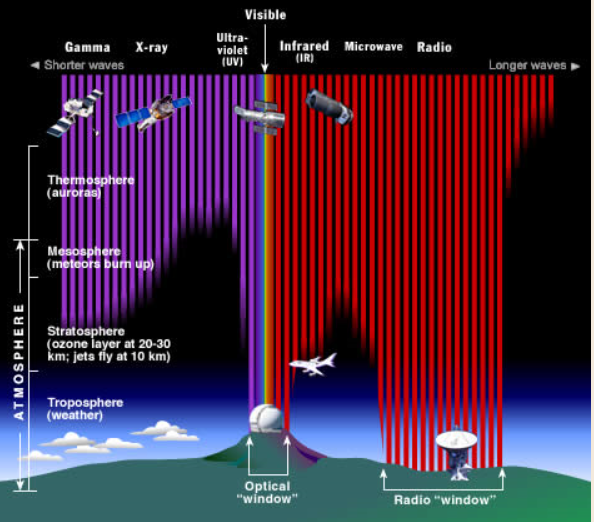
\includegraphics{images/durchlaessigkeit.png}
  \end{itemize}
\end{frame}

\end{document}

% quellen:
% https://www.slideshare.net/antglezatienza/galaxias-activas-87180963
% anderen bilder aus elsaessers script-> links von da besorgen